\section{Vorhersagen treffen}
\label{chap:Prediction}

Da nun ein Modell definiert und mit Daten angelernt wurde, sollen mögliche Vorhersagen zur Bewertung von Anwendungsregeln getroffen werden. 
Um die Anwendung des Modells vorzustellen, wurde vor dem Trainingsprozess eine Zeile aus dem Trainingsdatensatz entfernt. 
Das Modell soll nun zu dieser Zeile einen Vorschlag zur Bewertung abgeben. Zum Treffen von Vorhersagen kann 
die Methode predict() der Keras-Bibliothek benutzt werden. Mit dieser Methode können einem trainierten Modell neue Daten übergeben werden.
Anhand dieser Daten erstellt das Modell dann eine Vorhersage. Quellcode \ref*{lst:Predict} zeigt, wie so eine Vorhersage getroffen werden kann.
Da das Modell zwei Ausgabeschichten besitzt, gibt diese Methode auch zwei Objekte zurück. Diese Objekte sind Listen, welche die Wahrscheinlichkeiten
der einzelnen Ausprägungen beinhalten. Über diese Liste kann iteriert werden, um diese Wahrscheinlichkeiten auszugeben. Für den Statuswert 
wurden alle möglichen Ausprägungen ausgegeben, da dort nur drei Verschiedene vorhanden sind. Aufgrund der Übersichtlichkeit wird für das Statement
nur der Text ausgegeben, der die höchste Wahrscheinlichkeit besitzt. 
\begin{lstlisting}[language = python, caption={Vorhersage über neue Daten treffen},captionpos=b, label = lst:Predict, floatplacement=H]
    prediction_status, prediction_statement = model.predict(test)

    for val in prediction_status:
        for col in range(len(val)):
            print (str(trainYStatus.columns[col]) + " " + 
                   '{:.1%}'.format(val[col]))
    
    index_max = np.argmax(prediction_statement)
    for val in prediction_statement:
        print (trainYStatement.columns[index_max] + " " + 
               '{:.1%}'.format(val[index_max]))
\end{lstlisting}
Der tatsächliche Statuswert des Beispiels ist \glqq compliant\grqq{}. Die Ausgabe für den vorhergesagten Statuswert sieht wie folgt aus:
\begin{quotation}
    \noindent closed 2.0~\%\\
    compliant 88.2~\%\\
    not applicable 9.8~\%
\end{quotation}
Vergleicht man diese Ausgabe mit der Verteilung der Statuswerte der beispielhaft bewerteten Anwendungsregel in Abbildung \ref*{fig:StatusTest}, erkannt man eindeutig, 
dass das Modell eine Struktur erkennt und in der Lage ist, den Statuswert einer Anwendungsregel vorherzusagen.
\begin{figure}[H]
    \centering
    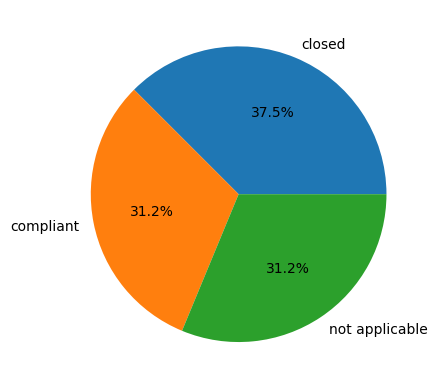
\includegraphics[width=.5\textwidth]{abbildungen/StatusTest.png}
    \caption{Verteilung des Statuswerts der betrachteten Anwendungsregel}
    \label{fig:StatusTest}
\end{figure}
\pagebreak
Das tatsächliche dazugehörige Statement lautet: 
\begin{quotation}
    \noindent Im Projekt ... sind die Signalkabel nach VDE0816/2 verwendet. Die Verlegevorschriften des Kabels sind beim Verlegen eingehalten. Daher ist diese Auflage erfüllt.  
    Bitte sieh  Kabelspezifikation (Aussenkabel)  A6Z00038004325  -  Outdoor Cable Plan  A6Z00037954383  -
\end{quotation}
Folgendes wurde vom Modell prognostiziert:
\begin{quotation}
    \noindent Zur Anschaltung der Weichen in der Außenanlage kommen Signalkabel nach  VDE 0816/2 oder Kabel mit vergleichbaren Eigenschaften zum Einsatz. Siehe  auch Dokument Requirement for 
    Signalling cable G68167-S0100-U-5009   A6Z08110839230  01.  20.8~\%
\end{quotation}
Wie bereits erwähnt, sind die meisten Statements einzigartig. Hier wurde jedoch ein Statement gewählt, welches vom Inhalt her identisch ist. Anhand der beiden vorhergesagten Attribute
kann geschlussfolgert werden, dass das Modell in der Lage ist eine Struktur beim Bewerten von Anwendungsregeln zu erkennen und Ähnlichkeiten in den Projekten festzustellen. Das war jedoch
nur ein Beispiel für eine bewertete Anwendungsregel. Im Anschluss gilt es noch, dieses Modell zu testen, im Idealfall mithilfe eines größeren Datensatzes.